\chapter{Theoretischer Teil}

\section{Virtuelle Maschinen} 
Die hier gesammelten Informationen wurden bei IBM\cite{vm} recherchiert. IBM ist mit RedHat ein Vorreiter auf diesem Bereich.\\
Als virtuelle Maschine bezeichnet man die Emulation einer physischen Maschine.
Durch Virtualisierung ist es möglich mehrere dieser \ac{VM}s auf einer Hardwaremaschine laufen zu lassen.
So können Maschinen mit verschiedenen Hardware-Eigenschaften, Betriebssystemen und Applikationen sich die zur Verfügung stehenden Ressourcen teilen, so dass sparsamer gearbeitet werden kann.

\subsection{Wie Virtualisierung funktioniert}
Eine \ac{VM} kann nicht direkt mit der ihr zugrunde liegenden Hardware kommunizieren. 
Sie benötigt dafür einen sogenannten Hypervisor.
Der Hypervisor ist eine dünne Softwareschicht, die auf dem Host läuft, und über die physische Ressourcen den einzelnen \ac{VM}s zugewiesen werden können.

Hypervisor lassen sich in zwei Typen einordnen:
\begin{itemize}
    \item Typ 1 \\ 
            Der Hypervisor wird direkt auf dem bare metal Server installiert, womit eine geringe Latenz und hohe Sicherheit garantiert werden.
    \item Typ 2\\
            Zwischen dem bare metal Server und dem Hypervisor ist eine \ac{OS} Schicht installiert. 
            Dieser Typ findet hauptsächlich bei Endnutzern Verwendung, die auf ihrer lokalen Maschine Virtualisierung betreiben wollen, zum Beipsiel um eine \ac{VM} zu testen bevor sie auf der eigentlichen Virtualisierungsumgebung ausgerollt wird.
            Durch die zusätzliche \ac{OS} Schicht ist die Latenz höher als beim ersten Typen.
\end{itemize}

Durch die Unabhängigkeit von der Hardware ist es möglich die \ac{VM}s problemlos zwischen verschiedenen Hosts zu verschieben. \\

\subsection{Vorteile von Virtuellen Maschinen}
Da sich durch diese Technologie mehrere Applikationen und Maschinen dieselben Ressourcen teilen können, ist das Arbeite mit \ac{VM}s deutlich Ressourcenschonender und effizienter als das Arbeiten mit klassischen hardware-Servern.
Durch den geringeren Verbrauch von Mitteln zahlt sich das Einsetzen auch aus finanzieller Sicht aus.
Des weiteren können die Server deutlich agiler gemanaged und vor allem auch schneller bereitgestellt werden.
Die Agilität führt auch dazu, dass Downtimes bei Umzügen oder Updates der Umgebungen reduziert werden.



\section{Container}
Die Informationen aus diesem Absatz stammen von Google\cite{containers}, einem der größten Innovatoren auf dem Bereich der Containertechnologien.
\subsection{Was ist ein Container?}
Unter einem Container verstehen wir ein vollständiges Paket, dass alle Bausteine enthält um eine bestimmt Applikation zu deployen.
Da alle Bestandteile in Ihm vereint sind ist das Deployment der Anwendung so komplett unabhängig von der zugrundeliegenden Umgebung, was den Prozess vereinfacht und verzulässiger macht.
Außerdem erlaubt es diese Isolierung der Applikation auch eine klare Grenze zwischen Anwendungsentwickler und Betrieb zu ziehen:
Der Entwickler kann sich darauf verlassen, dass seine Software immer unter den exakt gleichen Bedingungen ausgeführt wird, mit den gleichen Abhängigkeiten, den gleichen Software-Versionen und auf dem gleichen Betriebssystem.
\\
Der IT-Betrieb hingegen kann sich darauf verlassen, dass ein Container sich immer gleich verhält. 
Er muss für verschiedene Anwendungen keine unterschiedlichen Betriebssysteme und Software-Versionen installieren, sondern muss nur den Container managen.
\\
Container können also, wie auch \ac{VM}s, als isolierte Umgebungen betrachtet werden, sie sind allerdings deutlich kleiner.

\subsection{Vorteile von Containern}

Container virtualisieren auf \ac{OS}-Level und auf dem gleichen Kernel wie das \ac{OS}.
Dadurch können sie deutlich schneller gestartet werden und haben einen deutlich kleineren Overhead als \ac{VM}s, da sie kein komplett funktionsfähiges Betriebssystem benötigen um zu laufen.
Der komplette Speicherplatz-, CPU- und Arbeitsspeicher-Verbrauch des \ac{OS} wird somit an Ressourcen auf dem Host-System eingespart.

\subsubsection{Gleichbleibende Umgebung}
Da in dem Container immer von einer gleichbleibenden Umgebung ausgegangen werden kann, wird die Produktivität der einzelnen Entwicklern deutlich gestiegert.
Diese müssen sich, durch die Verwendung von Container-Technologien, nicht länger mit unterschiedlichen Umgebungsbedingungen auseinandersetzen und können sich auf das entwickeln neuer Featuren konzentrieren.

\subsubsection{Auf jeden System ausführbar}
Container sind auf fast jedem System ausführbar. 
Ob Linux, Mac, Windows, \ac{VM}s, Datacentern oder Bare Metal.
Dies wird nicht zuletzt durch das sehr populäre Docker Image Format gewährleistet, das überall sehr verbreitet ist. 

\subsubsection{Isolation}
Arbeitsspeicher, CPU und Speicher sind auf Betriebssystemebene virtualisiert und somit bis zu einem gewissen Level vom Rest des Systems abgegrenzt. 
Die Isolation ist jedoch weniger stark als bei \ac{VM}s.



\section{Vergleich von Virtuellen Maschinen und Containern}

Beide Technologien haben ähnliche Ziele: \\
Höhere Schnelligkeit und Agilität beim Bereitstellen von Software, geringere Downtimes und Einspraung von Ressourcen. \\
Durch die unterschiedliche Herangehensweise hat jede Technologie andere Anwendungsbereiche als Ziel, sowie andere Stärken.
Die zusätzliche \ac{OS}-Schicht, in Abbildung \ref{fig:comparison_vm_container} dargestellt, bringt zwar einen deutlich größeren Overhead mit sich, dafür aber auch bessere abgrenzen der einzelnen Applikationen voneinander.
Die wichtigsten Unterschiede sind in Tabelle \ref{table:comparison_vm_container} noch einmal zusammengefasst. 

\begin{table}[h]
        \centering
        \begin{tabular}{ | p{0.25\textwidth} | p{0.25\textwidth} | p{0.25\textwidth} | }
        Kategorie & Virtuelle Maschine & Container \\
        \hline \\
        Startup-Zeit & Im Minuten Bereich & Millisekunden bis Sekunden \\
        Performance & Großer Overhead, dadurch reltiv langsam & Kleiner Overhead, sehr schnell\\
        Operating System & Jede \ac{VM} kann auf einem unterschiedlichen \ac{OS} laufen & Alle Container teilen sich das \ac{OS} des Hosts \\
        Operations & Anpassungen müssen auf den \ac{VM}s vorgenommen werden. Unterschiedliche Maschinen, welche dieselbe Applikation bereitstellen können sich somit trotzdem unterscheiden. & Durch die deklarative Natur der Containertechnologien müssen keine Administratoren den Containern arbeiten. Anpassungen werden ausschließlich in den Images und Dockerfiles vorgenommen. Der Administrative Aufwand ist sehr gering. \\
        \end{tabular}
        \caption{Unterschiede von VM's und Containers}
        \label{table:comparison_vm_container}
\end{table}

\begin{figure}[h]
        \caption{Vergleich von Virtuellen Maschinen und Containern\cite{vm_vs_container}}
        \centering
        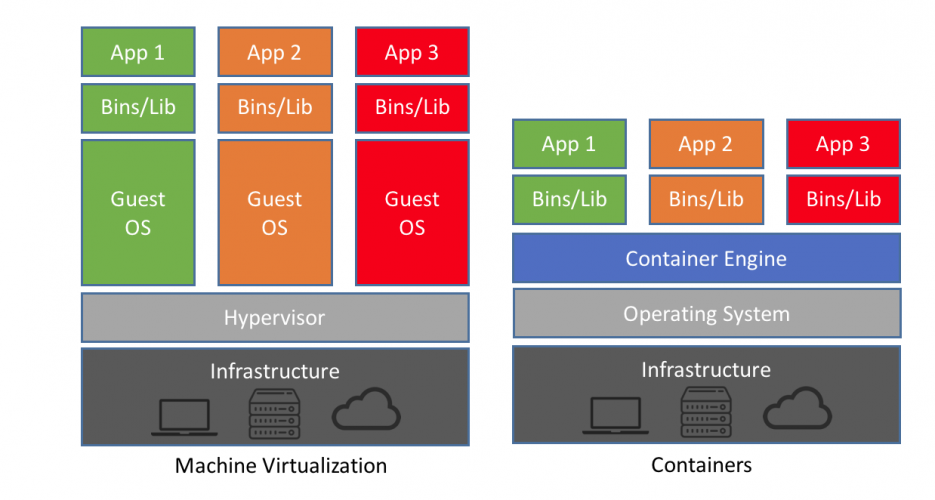
\includegraphics[width=0.8\textwidth]{bilder/comparison_vm_container.png}
        \label{fig:comparison_vm_container}
\end{figure}



\section{Open Container Initiative}
Die \ac{OCI} ist eine Organisation, die Standarts für Container Runtimes und Formate erstellt.
Aktuell werden zwei Spezifikationen von der Organisation bereitgestellt, die \ac{runtime-spec} und die \ac{image-spec}.
Die Spezifikationen erlauben es verschiedener Software, das bereitgestellt Interface zu implementieren.
Die \ac{runtime-spec} definiert wie ein Container auf dem Hsot ausgeführt werden muss. 
Eine \ac{OCI}-Implementation, wie zum Beispiel Docker, lädt zum Ausführen eines Contaienrs ein \ac{OCI}-kompatibles Container-Image herunter und entpackt dieses in ein Runtime Filesystem Bundle.
Ohne die Definitionen des \ac{OCI} könnte ein Container der im Docker-Format und die Docker-Runtime(runc) geschrieben wurde auch nur von Docker ausgeführt werden.
Die \ac{OCI}-Spezifikation ermöglicht es, mit jeder Container-Runtime, die \ac{OCI}-kompatibel ist, ein Docker-Image auszuführen. \cite{oci}



\section{Kata-Runtime}
Das Kata Containers Projekt ist ein Open Sorce Projekt, das probiert die Vorteile beider zuvor erläuterten Technologien zu kombinieren.
Die Isolation von \ac{VM}s mit der Geschwindigkeit, dem geringen Management Aufwandt und dem Self-Healing von Contaienern.
\\
Wenn ein Contaienr-Image in der Kata-Runtime gestartet wird, wird tatsächlich kein Container gestartet, sondern eine lightweight \ac{VM} erstellt.
Diese hat ihren eigenen Kernel, der eine Isolation des Netzwerks, des Speichers und von \ac{I/O} garantiert, jedoch mit einem deutlich kleineren Overhead als konventionelle \ac{VM}s.
Um einen möglichst großen Anwenderbereich abzudecken arbeitet Kata nach den Industrienne Standarts \ac{OCI} und implementiert Kubernetes \ac{CRI}, das im Verlauf der Arbeit noch genauer gerklärt wird. 
Durch die standatisierten Interfaces ist der Umstieg und das Arbeiten mit Kata in der Theorie sehr unkompliziert. \cite{kata}

\subsection{Geschichte}
Das Kata-Container Projekt entstand aus der Fusion von zwei vorhergehenden Projekten:
\begin{itemize}
        \item Clear Contaienrs
        \\Dieses Projekt von Intel\footnote{https://www.intel.com/content/www/us/en/homepage.html} wurde 2015 ins Leben gerufen, um Sicherheitsbedenken beim Einsatz von Containern aus dem Weg zu räumen.
        Intel erschuf eine alternative Container Runtime, in der Container als minimale \ac{VM}s gestartet wurden, den Focus setzten sie dabei auf Performance(<100ms boot time) und Sicherheit.\cite[S.1]{Kata_Containers}
        \item runv
        \\Ist ein ähnliches Projekt von der Firma "Hyper", die selbst eine Runtime entwickelt haben, die einen Hypervisor nutzt.
        Sie haben Ihren Fokus auf den Support vieler CPU-Architekturen und Hypervisor gelegt.\cite[S.1]{Kata_Containers}
\end{itemize}
2016 hielten beide Firmen eine Presentation über ihr jeweiliges Produkt auf der "Open Source Summit" in Berlin und wurden so aufeinander aufmerksam.
Ein Jahr später, in 2017, wurde beide Produkte unter der \ac{OSF} zu Kata-Containers zusammengeführt.\cite{kata_history}

\subsection{Vergleich mit traditionellen Containern}

\begin{figure}[h]
        \caption{Vergleich von Kata-Containern und traditionellen Containern\cite{kata_learn}}
        \centering
        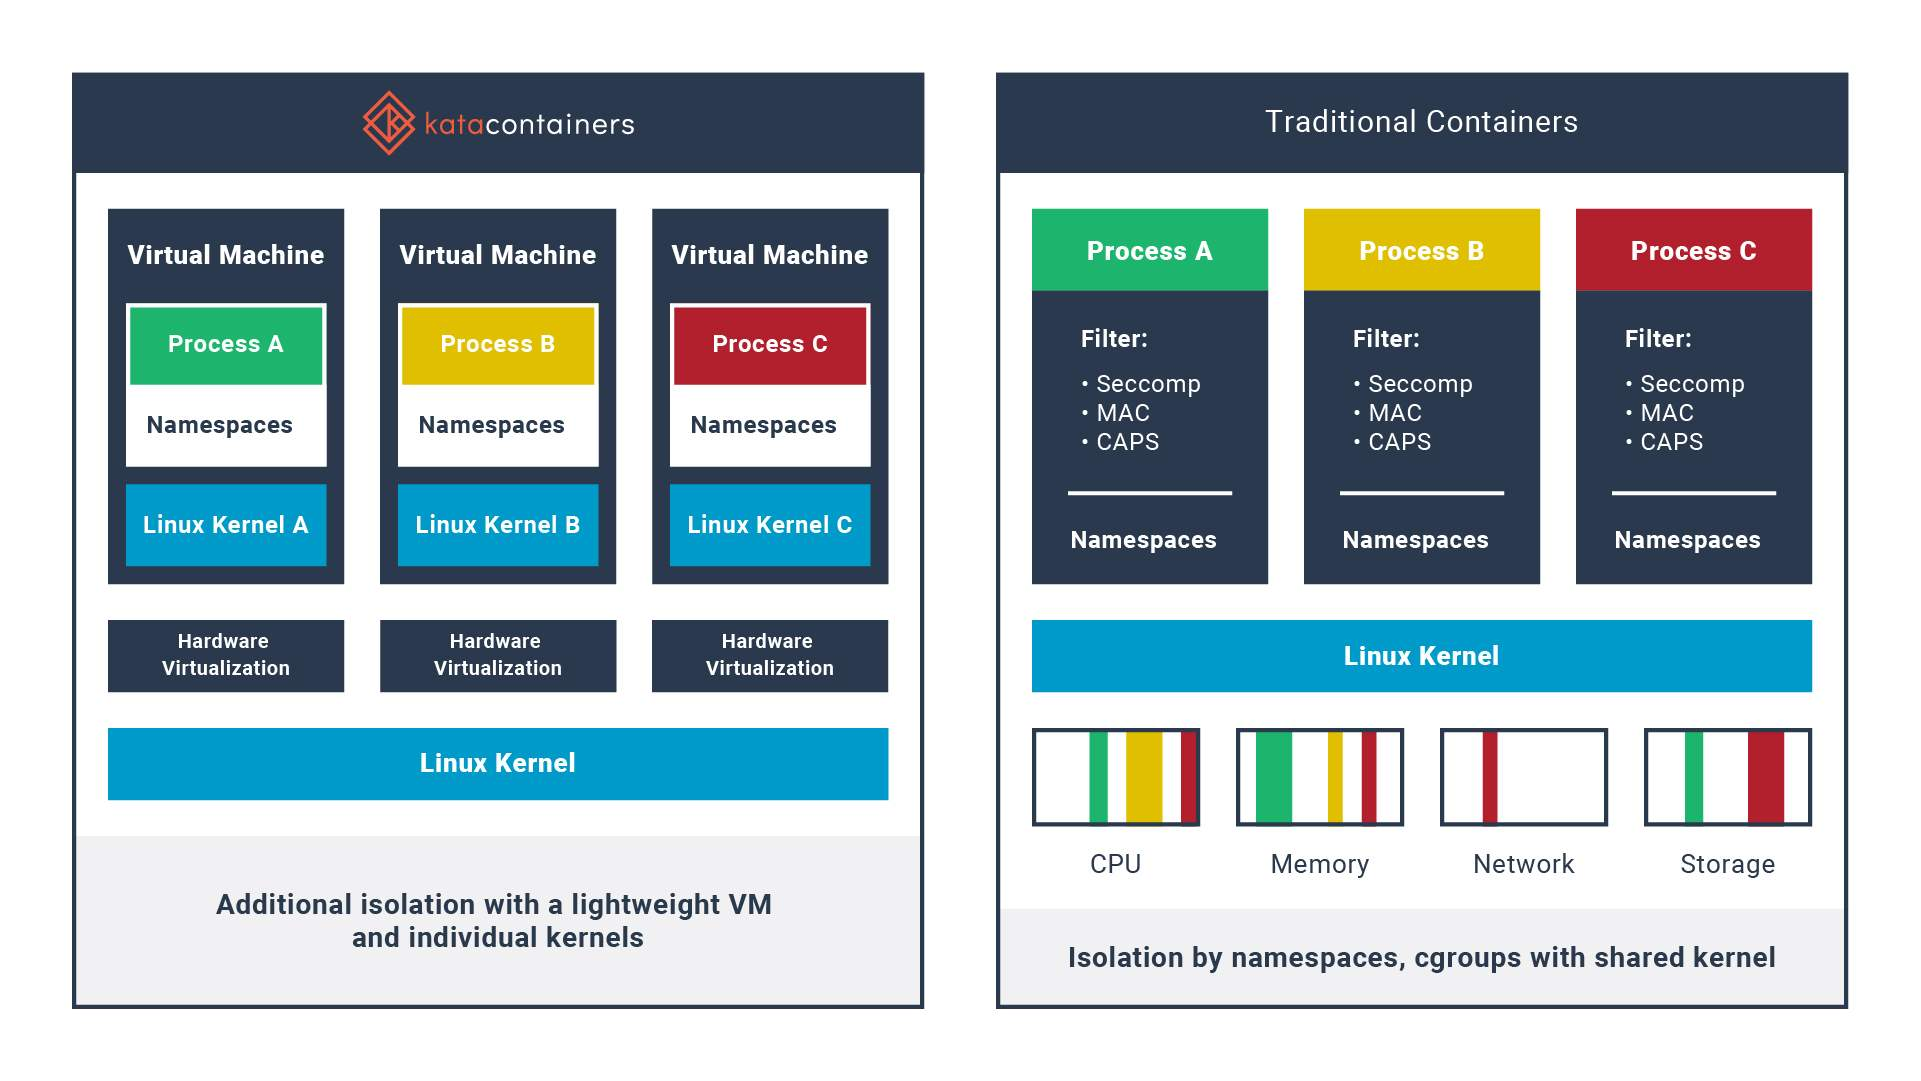
\includegraphics[width=\textwidth]{bilder/katacontainers_traditionalvskata_diagram.jpg}
        \label{fig:kata_vs_traditional}
\end{figure}

In der Abbildung \ref{fig:kata_vs_traditional} werden die wichtigsten Unterschiede dargestellt.
Traditionelle Container laufen alle auf demselben Kernel. 
Das bedeutet, dass jeder Container direkt auf den Ressourcen(CPu, Memory, Network, Storage) des Hosts läuft. 
Eine Isolation wird durch Namespaces und cgroups realisiert.
\\
Bei den Kata-Containern hingegegen werden die Container in \ac{VM}s verpackt, von denen jede seinen eigenen Kernel bekommt.
Durch die Hardware-Virtualisierung kann jeder container nur auf die Ressourcen zugreifen, welche für ihn erstellt wurden. 
In seinem Kernel laufen keine Prozesse, außer diejenigen der Applikation selbst.  



\todo{Weiter ausführen mit Grafiken}



\section{Kubernets}
Kubernetes ist eine \ac{FOSS}-Lösung zum managen von containerisierten Anwendungen.
Das System ermöglicht automatisches Skalieren und Deploymen der Anwendungen, sowie integriertes Self-Healing, einfaches Management und Updaten.
Außerdem ist es vergleichsweise unproblematisch ein Kubernetes-Cluster selbst zu skalieren. 
Nodes lassen sich im Live-Betrieb nicht nur hinzufügen, sondern können genauso auch ausfallen. 
Die auf ihnen laufenden Container werden dann, wenn möglich ohne Downtimes, auf die verbliebenen zur Verfügung stehenden Nodes verteilt. 
Gehostet werden kann Kubernetes sowohl on-premise als auch in der public- oder hybrid-cloud.
\\
Entwickelt wurde die Technologie ursprünglich von Google, die schon seit 15 Jahren Produktions-Arbeitslast in Containern laufen lassen.
\cite{kubernetes}
\todo{Mit Buch als Quelle vervollständigen}




\section{Ansible}
Ansible ist eine Software, mit dessen Hilfe Systeme deployed und gemanaged werden können. 
Dazu wird ein Prozess, der eigentlich händisch ausgeführt werden würde, in einem sogenannten Playbook abgebildet.
Dieses Playbook beschreibt der Reihe nach genau jede Bedindung die erfüllt sein muss, um den Prozess abzuschließen.
Durch die deklarative Natur von Ansible sind die Ergebnisse reproduzierbart und führen nur die Änderungen aus, die nötig sind.
Wird ein wiederkehrendes Problem einmal in einem Ansible-Playbook gelöst, kann dieses Playbook immer wieder Verwendung finden, wenn das Problem erneut auf einem ähnlichen System auftritt.
Ansible lässt sich auch einsetzen, um den Umgang mit bereits eingesetzten Technologien zu vereinfachen oder zu automatisieren.
\cite{ansible}

\subsection{Funktionsweise}
Ansible ermöglicht es, die gesamte Infrastruktur mitsamt all ihren Verbindungen zu beschreiben. 
So kann die ganze Umgebung, statt nur einzelne Systeme, auf einmal angepasst werden.
Dazu nutzt Ansible die bereits angesprochenen Playbooks, die in \ac{YAML} geschrieben sind, einer deklarativen und sehr simpel gestalteten Sprache.
\\
Wird ein Playbook ausgeführt stellt Ansible auf den einzelnen Systemen mithilfe von einigen "Modulen" den gewünschten Stand her, und löscht diese Module anschließend wieder. 
Um die Verbindungen zu den einzelnen Systemen herstellen zu können nutzt die Software standartmäßig \ac{SSH}-Keys, es sind allerdings auch andere Identity-Management Systene wie z.B. Kerberos unterstützt.
Die Systeme selbst werden in den Inventory Files aufgelistet und können mit Gruppen und Variabeln ausgestattet werden, um in einer Infrastruktur beispielsweise nur die Webserver oder nur die Datenbank-Server anzusprechen.
Wird ein OpenStack oder Ähnliches als Infrastruktur genutzt, kann sogar ein dynmaisches Inventory generiert werden.
\cite{how_ansible_works}
\\
In diesem Projekt soll Ansible verwendet werden, um einen reproduzierbaren Weg zum installieren und konfigurieren der Kata-Runtime zu finden, sowie um das Kubernetes Cluster aufzubauen und zu managen. 


\section{Helm}
Helm ist eine Software, die das Installieren und Updaten von komplexen Kubernetes Aplikationen vereinfachen soll.
Helm-Charts sind einfach zu erstellen, sie bieten eine gute Versionierung, lassen sich veröffentlichen und teilen, sowie templaten.
Das Projekt ist ein \ac{CNCF}-Projekt und wird von der Community gepflegt.
Charts beschreiben komplexe Applikationen und ermöglichen somit eine vereinfachte Installation von umfangreicher Software, außerdem sind diese einfach zu teilen und somit ein guter Weg um Software zu veröffentlichen.
\cite{helm}
\\
Für das \ac{SORMAS}-Projekt wird Helm jedoch auch vor allem wegen der guten Templating Möglichekeiten eingesetzt.
Verchiedene \ac{GAs} benötigen unterschiedliche Attribute, die alle über das Helm-Templating gesetzt werden könne.
So kann garantiert werden, dass nur an einer einzigen Stelle im Code jemals Anpassungen gemacht werden müssen, wenn eine neue \ac{SORMAS-ÖGD}-Instanz ausgerollt werden soll.

